\documentclass[tikz,border=10pt]{standalone}
\usetikzlibrary{calc}

\begin{document}
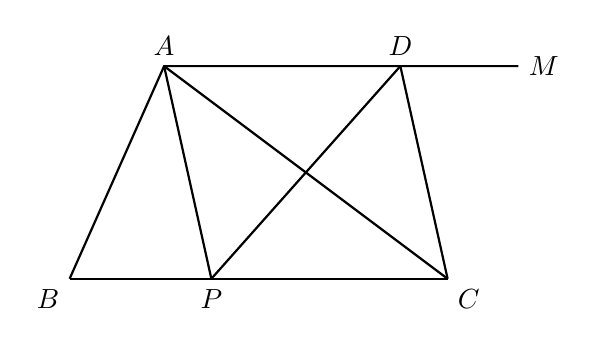
\begin{tikzpicture}[thick, scale=1.5]
    % 1. 定义坐标 (基于平行四边形布局)
    \coordinate (B) at (0,0);
    \coordinate (A) at (0.8,1.8);
    \coordinate (C) at (3.2,0);
    \coordinate (P) at (1.2,0); % P点在BC中间的位置
    \coordinate (D) at (2.8,1.8);
    \coordinate (M) at (3.8,1.8); % 射线AD的延长方向

    % 2. 绘制图形边框
    \draw (B) -- (A) -- (M); % 上方边界及延伸
    \draw (B) -- (C);        % 下方基准线
    \draw (A) -- (P);        % 内部连接AP
    \draw (P) -- (D);        % 内部连接PD
    \draw (A) -- (C);        % 内部连接AC
    \draw (C) -- (D);        % 右侧边界线

    % 3. 标注点名
    \node[below left] at (B) {$B$};
    \node[above] at (A) {$A$};
    \node[below] at (P) {$P$};
    \node[below right] at (C) {$C$};
    \node[above] at (D) {$D$};
    \node[right] at (M) {$M$};

\end{tikzpicture}
\end{document}